\chapter{Fundamentos teóricos} \label{chap:fundamentos-teoricos}

En este Capítulo vamos a dar una introducción a los algoritmos de aprendizaje automático que más adelante usaremos para realizar nuestro análisis con datos reales de laboratorio.

En la Sección \ref{sec:unsupervised} vamos a tratar algunos algoritmos no supervisados, tanto para la reducción de la dimensión de los datos y su visualización, como para la agrupación de los datos en distintas clases, con un número de ellas tanto preestablecido como generado automáticamente a partir de ellos. Posteriormente, en la Sección \ref{sec:supervised} vamos a introducir algoritmos de clasificación supervisada centrándonos en las redes neuronales, tanto secuenciales como convolucionales.

\section{Métodos no supervisados}
\label{sec:unsupervised}

Los algoritmos de aprendizaje automático no supervisados se utilizan cuando no se conoce la salida esperada. Al algoritmo de aprendizaje se le otorgan los datos de entrada y se le pide extraer información de estos datos. Las principales aplicaciones de estos algoritmos, las cuales vamos a aprovechar, son la agrupación de datos y la reducción de dimensionalidad de las variables de los mismos. Esa última es usada principalmente para poder hacer representaciones de datos multidimensionales, los cuales serian complejos de visualizar de otra forma.

La principal pega que pueden tener estos algoritmos es que, si bien no siempre son capaces de identificar conocimiento dados los datos utilizados, cuando lo obtienen, no siempre es el conocimiento que esperábamos obtener. Póngase el ejemplo de un algoritmo que tratase de agrupar rostros de personas iguales. Al no darle a priori ningún tipo de salida de ejemplo, el algoritmo puede acabar clasificando si los rostros están de frente o de lado, no precisamente lo que esperábamos. Es por ello que estos algoritmos cuentan con diversidad de parámetros para ajustarlos a nuestras necesidades, tratando de realizar la agrupación deseada.

En esta sección vamos a estudiar a fondo tres tipos de algoritmos de agrupación: el agrupamiento por k-medias, el agrupamiento aglomerativo, y el agrupamiento por afinidad. Además, estudiaremos también el principal algoritmo de reducción de dimensiones, el análisis de componentes principales, PCA, de sus siglas en inglés. Los principales ejemplos y explicaciones de los algoritmos han sido inspirados por los dados en \cite{machine}.

\begin{mypython}[float={h}, caption={Generar datos artificiales de prueba.}, label={code:artificial-data}]
  from sklearn.datasets import make_blobs

  X, y = make_blobs(n_samples=100, centers=4,
                  n_features=3, random_state=0)
\end{mypython}

Hemos creado un conjunto de datos sintéticos a los cuales poder aplicar todos los algoritmos que vamos a explicar para poder visualizar gráficamente sus resultados. Con la función \texttt{make\_blobs} de Scikit-learn hemos aleatorizado 100 puntos tridimensionales agrupados en cuatro clases fácilmente diferenciables. La figura \ref{fig:artificial-data} muestra una representacion gráfica del conjunto, y el Código \ref{code:artificial-data}. En la tabla \ref{tab:colab-links} está el enlace para poder ejecutar el código en el \textit{backend} de Google.

% Artificial data
\begin{figure}[h]
  \centering
  \begin{subfigure}{0.45\textwidth}
    \centering
    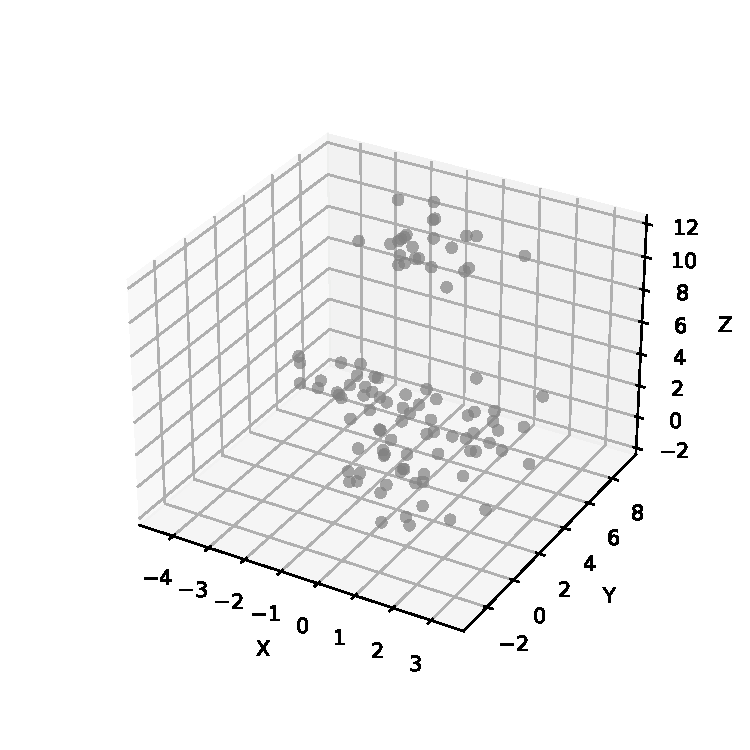
\includegraphics[width=\textwidth]{figures/artificial-data.pdf}
    \caption{}
    \label{fig:artificial-data-grey}
  \end{subfigure}
  \begin{subfigure}{0.45\textwidth}
    \centering
    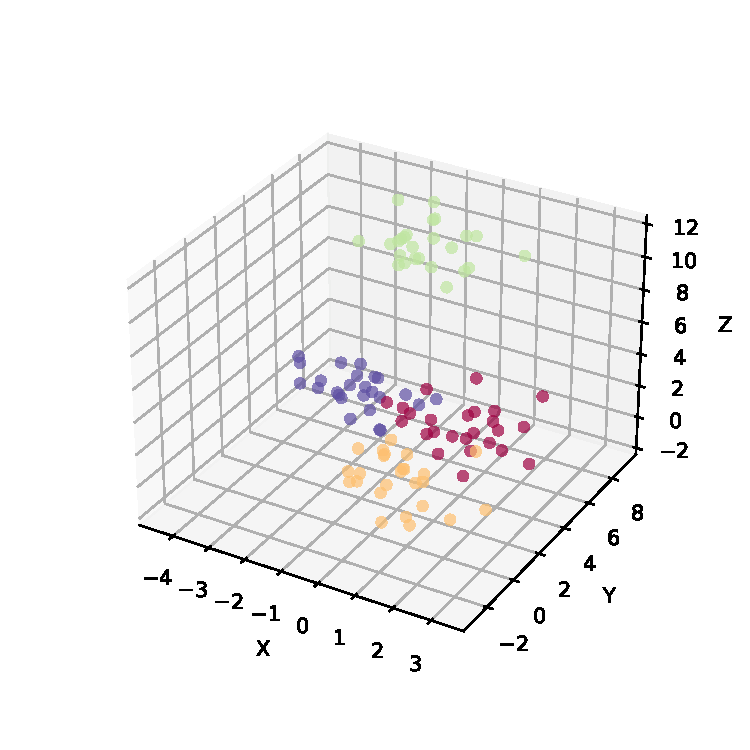
\includegraphics[width=\textwidth]{figures/artificial-data-labeled.pdf}
    \caption{}
    \label{fig:artificial-data-labeled}
  \end{subfigure}
  \caption[Datos artificiales para la prueba de algoritmos.]{Datos artificiales generados para probar algoritmos de agrupamiento. Consisten en 100 puntos tridimensionales agrupados equilibradamente al rededor de 4 centros aleatorios. \ref{fig:artificial-data-grey} En gris los puntos generados sin asignar ninguna etiqueta. Estos serán los datos que recibirán los algoritmos para procesar y agrupar. \ref{fig:artificial-data-labeled} Datos etiquetados según el grupo al que pertenecen. Esto nos ayudará a verificar la eficacia de nuestros algoritmos.}
  \label{fig:artificial-data}
\end{figure}

\subsection{Análisis de componentes principales}

Nuestro conjunto de datos artificiales tiene únicamente 3 dimensiones, lo que hace que sea sencillo poder representarlo gráficamente y que sea fácilmente interpretable. Sin embargo, en la vida real, así como en los datos que en el Capítulo \ref{chap:analisis-y-experimentacion}, los datos tienden a tener muchas más dimensiones. Esto hace que sea un problema poder representarlos en espacios bidimensionales como este documento, y puede entorpecer también su interpretación o lectura desde otros algoritmos, ya que es probable que haya dimensiones que aporten más ruido que información a la muestra.

Una de las técnicas más utilizadas para tratar este problema es realizar un análisis de componentes principales (PCA) sobre los datos \cite{pca}. Un PCA es una transformación lineal de los datos a un nuevo sistema de coordenadas para facilitar la identificación de las direcciones que contienen más variabilidad. A estas direcciones, que consisten en una combinación lineal de las variables originales, se les denomina \textit{componentes principales}.

El primer paso para realizar un PCA es normalizar los datos para que cada una de las variables originales tenga media 0 y varianza 1. Para ello, denotando $ \textbf{X} = (X_1, ..., X_n) $ a nuestros datos a analizar, donde cada $ X_i $ con $ i \in {1, ..., n} $ es una de las variables de nuestros datos, y $ \mu_{X_i} $ y $ \sigma_{X_i} $ son la media y varianza de cada una de las variables, computamos
\begin{equation}
  Z_i = \frac{X_i - \mu_{X_i}}{\sigma_{X_i}},
\end{equation}
para cada $ i $, obteniendo $ \textbf{Z} = (Z_1, ..., Z_n) $ el conjunto de todas nuestras variables normalizadas. Con esto se estandariza la escala de las variables de nuestros datos, evitando que las variables con escalas mayores dominen al resto. En el Código \ref{code:standar} realizamos la normalización de nuestros datos artificiales utilizando la clase \texttt{StandardScaler} de Scikit-learn.

\begin{mypython}[float={h}, caption={Escalar y estandarizar los datos.}, label={code:standar}]
  from sklearn.preprocessing import StandardScaler

  scaler = StandardScaler()
  scaler.fit(X)
  Z = scaler.transform(X)
\end{mypython}

Una vez todos nuestros datos están en la misma escala estamos en disposición de realizar el PCA propiamente dicho. Para ello calculamos la matriz de covarianza $ \Sigma $ de nuestros datos normalizados. $ \Sigma $ es una matriz de dimensión $ n \times n $ con
\begin{equation}
  \Sigma_{ij} = \operatorname{Cov}(Z_{i},Z_{j}) = E[Z_{i}Z_{j}] - E[Z_{i}] E[Z_{j}],
\end{equation}
para $ i, j \in {1, ..., n} $ siendo $ E $ el operador media. Acto seguido, calculamos los $ n $ pares de autovalores y autovectores de la matriz $ \Sigma $ resolviendo la ecuación
\begin{equation}
  \Sigma \textbf{v} = \lambda \textbf{v}.
\end{equation}

Los autovectores $ \textbf{v} $ se denominan componentes principales, y ordenándolos en orden decreciente según el valor de su autovalor $ \lambda $ asociado, obtenemos la lista de componentes principales deseada. Finalmente basta con quedarse con el numero deseado de componentes de la parte superior de la lista para reducir la dimensionalidad de nuestros datos maximizando la covarianza de los mismos. En el Código \ref{code:pca} hemos realizado un PCA de nuestros datos artificiales conservando las 3 componentes principales. Hemos utilizado la clase \texttt{PCA} de Scikit-learn, que encapsula todo el procedimiento que hemos explicado. 

\begin{mypython}[float={h}, caption={Realizar un PCA.}, label={code:pca}]
  from sklearn.decomposition import PCA

  pca = PCA(n_components=3)
  pca.fit(Z)
  Z_pc = pca.transform(X)
\end{mypython}

En la Figura \ref{fig:pca} se muestran gráficamente los puntos artificiales tras el anális de componente principales.

% PCA
\begin{figure}[]
  \centering
  \begin{subfigure}{\textwidth}
    \centering
    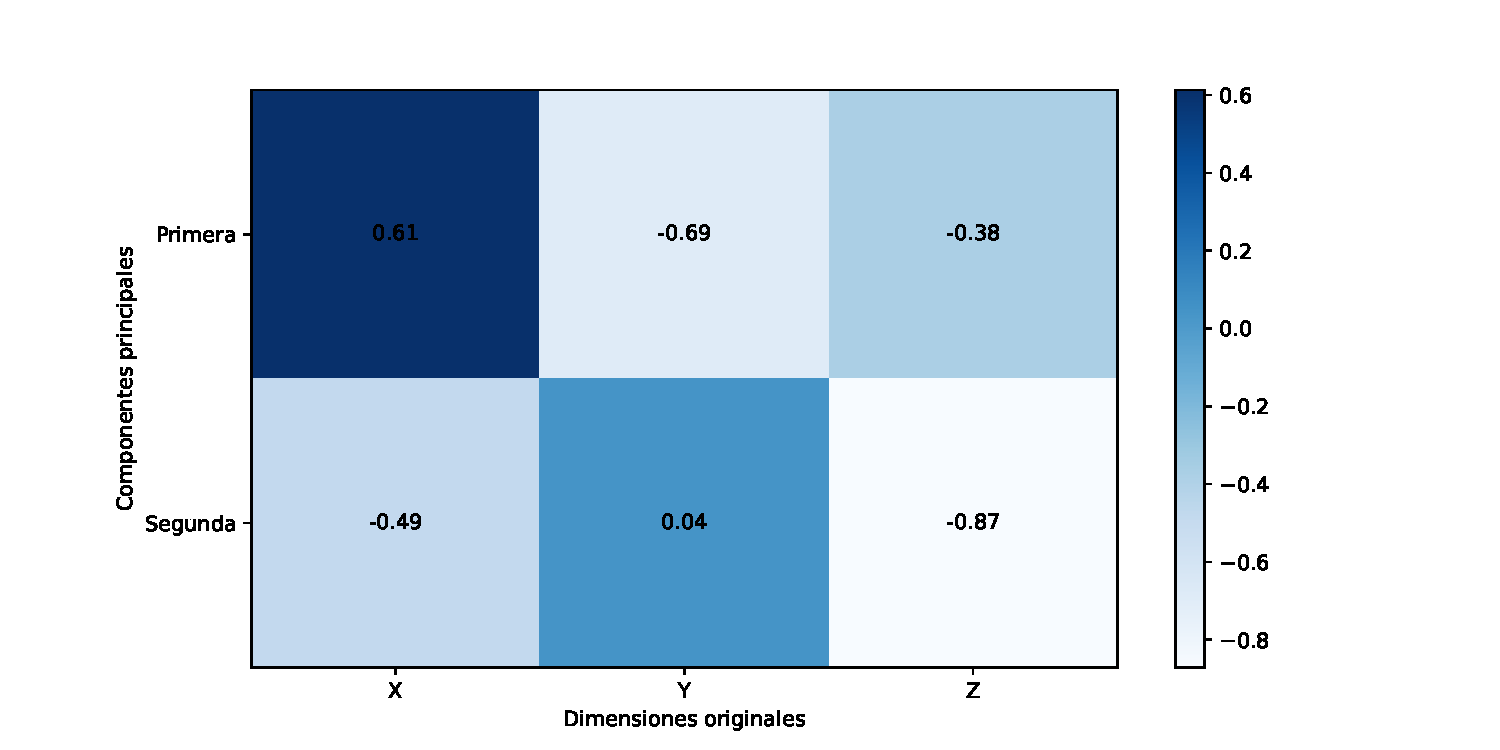
\includegraphics[width=\textwidth]{figures/pca-color-ponderation.pdf}
    \caption{}
    \label{fig:pca-color-ponderation}
  \end{subfigure}
  \begin{subfigure}{0.45\textwidth}
    \centering
    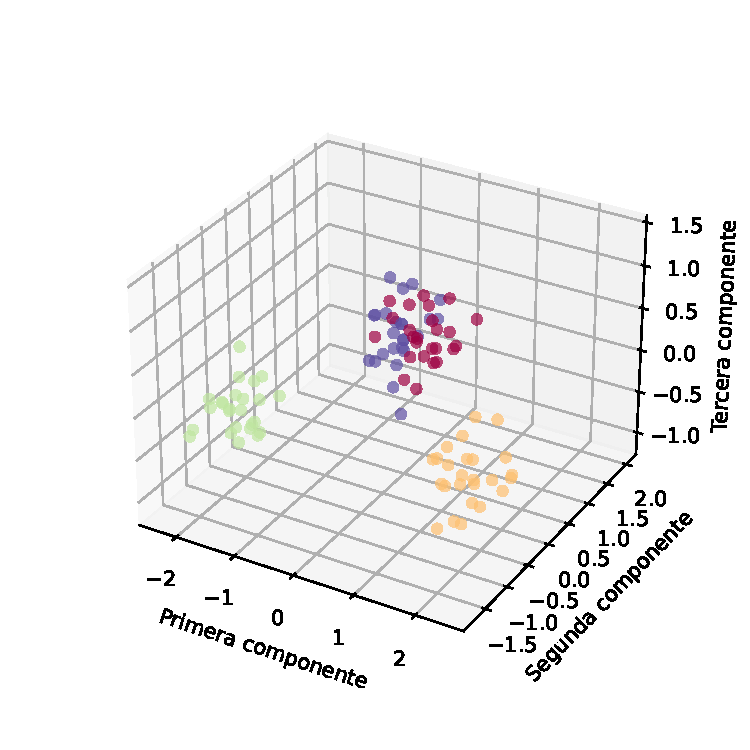
\includegraphics[width=\textwidth]{figures/pca-3d-labeled.pdf}
    \caption{}
    \label{fig:pca-3d-labeled}
  \end{subfigure}
  \begin{subfigure}{0.45\textwidth}
    \centering
    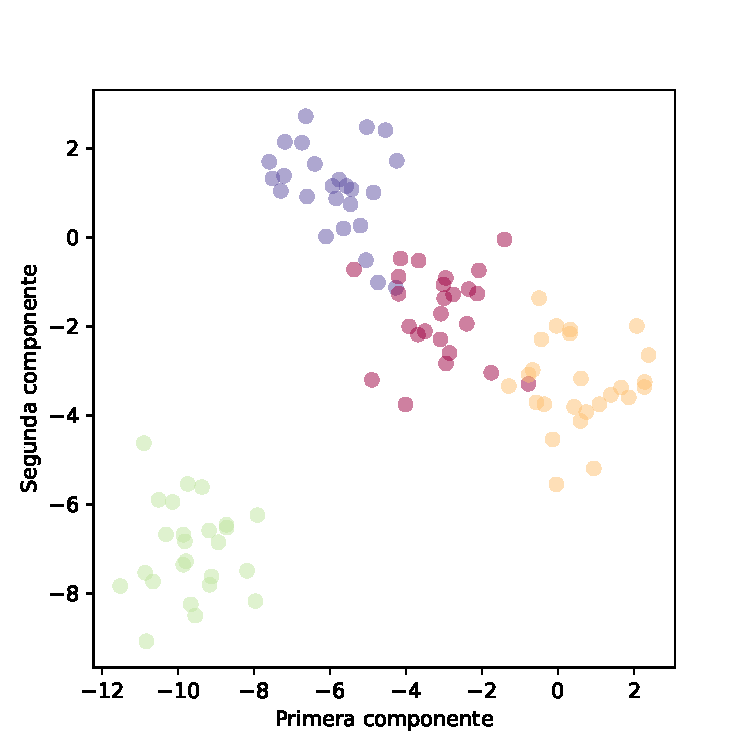
\includegraphics[width=\textwidth]{figures/pca-labeled.pdf}
    \caption{}
    \label{fig:pca-labeled}
  \end{subfigure}
  \caption[Prueba del algoritmo de PCA.]{Prueba del algoritmo de PCA. \ref{fig:pca-color-ponderation} Mapa de calor con las ponderaciones asignadas por el PCA a cada uno de las dimensiones originales. \ref{fig:pca-3d-labeled} Visualización de los datos previamente generados tras escalarlos y aplicarles la PCA. Los colores de los grupos se mantienen, pero los ejes ahora representan las componentes principales, en vez de las dimensiones originales. \ref{fig:pca-labeled} Visualización de las dos primeras componentes principales sobre el plano. Este será el formato en el que visualizaremos más adelante las agrupaciones ejercidas sobre datos reales de dimensionalidad alta.}
  \label{fig:pca}
\end{figure}

\newpage
\subsection{Agrupamiento por k-medias}

El algoritmo de k-medias clasifica los datos separando los datos en $ n $ grupos con la misma varianza.

El algoritmo comienza inicializando aleatoriamente $ n $ centroides, siendo $ n $ el número de agrupaciones que se le han dicho que realice. Estos centroides serán los centros de las agrupaciones que va a realizar, no tienen por qué pertenecer a los datos, pero sí que están contenidos en su misma dimensión. En cada iteración, el algoritmo asigna a cada punto de los datos el centroide más próximo y luego asigna a cada agrupación un nuevo centroide calculado como la media de los datos que se han asignado a dicha agrupación.

El algoritmo divide un conjunto de $ n $ puntos $ x_i $ en $ j $ agrupaciones disjuntas $ C $, cada una descrita por la media $ \mu_j $ de los puntos en la agrupación. Para ello se computan los centroides que minimicen
\begin{equation}
  \sum\limits_{i=1}^n \underset{\mu_j \in C}{\operatorname{min}} (|| x_i - \mu_j||^2).
\end{equation}

Cuando una iteración no realiza ninguna modificación de las agrupaciones generadas por los centroides de la iteración anterior, el algoritmo finaliza devolviendo las agrupaciones cradas asignando una clase a cada uno de los puntos procesados.

Para computar el algoritmo sobre nuestros datos artificiales hemos utilizado el Código \ref{code:kmeans} usando la clase \texttt{KMeans} de Scikit-learn. Hemos iniciado al algoritmo que separe los datos en dos clases, iniciando los centroides de forma automática. Con esto queremos ver como actúa un algoritmo dividiendo un conjunto de datos generado con 4 clases en mente, cuando se le fuerza a separar únicamente dos grupos.

\begin{mypython}[float={h}, caption={k-medias.}, label={code:kmeans}]
  from sklearn.cluster import KMeans

  kmeans = KMeans(n_clusters=2, n_init="auto")
  kmeans_assigment = kmeans.fit_predict(Z)
\end{mypython}

La Figura \ref{fig:kmeans} muestra las dos agrupaciones que se han decidido crear sobre los datos artificiales, simulando lo que más adelante haremos con los datos reales.

% k-means
\begin{figure}[h]
  \centering
  \begin{subfigure}{0.45\textwidth}
    \centering
    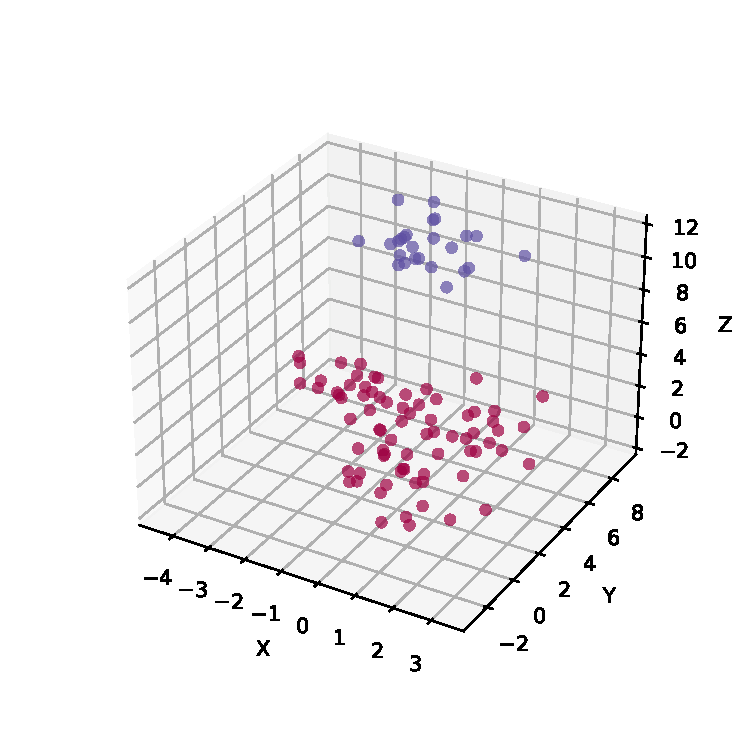
\includegraphics[width=\textwidth]{figures/kmeans-3d.pdf}
    \caption{}
    \label{fig:kmeans-3d}
  \end{subfigure}
  \begin{subfigure}{0.45\textwidth}
    \centering
    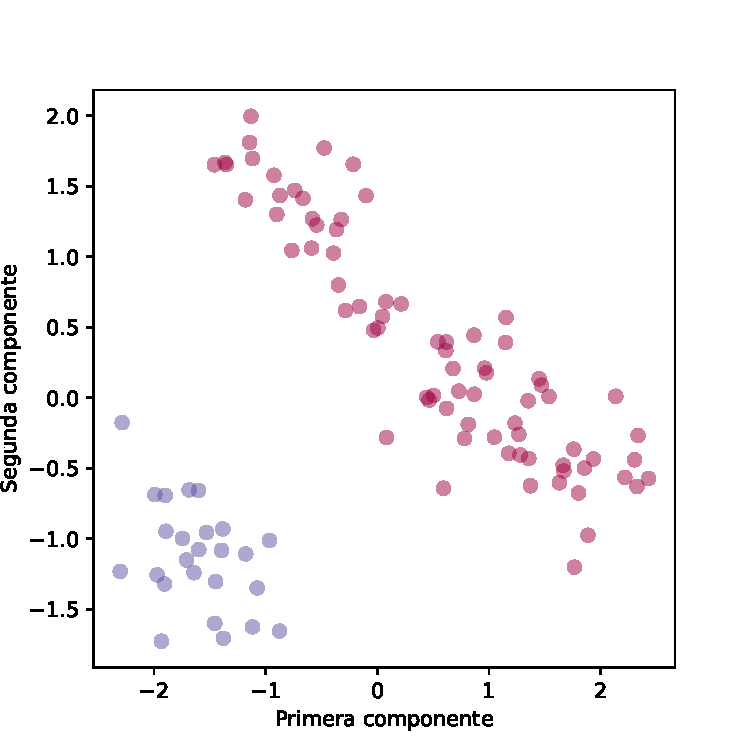
\includegraphics[width=\textwidth]{figures/kmeans-pca.pdf}
    \caption{}
    \label{fig:kmeans-pca}
  \end{subfigure}
  \caption[Prueba del algoritmo de k-medias.]{Prueba del algoritmo de k-medias. \ref{fig:kmeans-3d} Visualización sobre los datos sin modificar de los grupos que ha realizado el algoritmo de k-medias. \ref{fig:kmeans-pca} Visualización de los grupos realizados sobre los datos procesados por el PCA.}
  \label{fig:kmeans}
\end{figure}

\newpage
\subsection{Agrupamiento aglomerativo}

Al igual que el algoritmo de k-medias, el algoritmo de agrupamiento aglomerativo divide los datos dados en el número de grupos indicado. Para ello empieza asignando a cada punto un grupo diferente, para luego ir unificando los grupos en cada iteración según el criterio elegido, hasta alcanzar el número de grupos deseado. Este tipo de algoritmo pertenece a un tipo más amplio de algoritmos denominado agrupación jerárquica, donde además de los agrupamientos aglomerativos están las agrupaciones divisivas. Estas funcionan asignando a todos los puntos el mismo grupo y dividiendo este grupo en cada iteración hasta alcanzar el número deseado.

Los dos tipos de agrupamiento jerárquico funcionan de forma similar, y ambos varían dependiendo de la función de distancia que se utilice, tanto para dividir como para agrupar. Vamos a profundizar en el Método de Ward, que junta los grupos que al juntarse minimicen la varianza mínima dentro del nuevo grupo. Así, la varianza de un grupo $ C $ de puntos $ \{x_1, ..., x_m\} $ se define como
\begin{equation}
  V(C) = \sum\limits_{i=1}^n || x_i - \mu_C ||^2,
\end{equation}
siendo $ \mu_C $ la media de los puntos del grupo $ C $.

Por tanto, en cada iteración el algoritmo calcula el incremento de varianza que supondría juntar cada par de grupos $ A $ y $ B $ calculando
\begin{equation}
  \delta(A, B) = \frac{|A||B|}{|A|+|B|}||\mu_A - \mu_B||^2,
\end{equation}
donde $ |\cdot| $ denota el cardinal de los grupos y $ || \cdot || $ la operación módulo.

Tras ello, unifica los dos grupos que supongan un menor incremento en la varianza y repite el proceso hasta obtener el número deseado de grupos.

\begin{mypython}[float={h}, caption={Agrupamiento aglomerativo.}, label={code:agglomerative}]
  from sklearn.cluster import AgglomerativeClustering

  agg = AgglomerativeClustering()
  agg_assigment = agg.fit_predict(Z)
\end{mypython}

En el Código \ref{code:agglomerative} hemos realizado un agrupamiento aglomerado sobre nuestros puntos artificiales utilizando la clase \texttt{AgglomerativeClustering} de Scikit-learn, que por defecto, si no se le indica lo contrario, utiliza el Método de Ward en la ejecución del algoritmo. En la Figura \ref{fig:agglomerative} se muestran los resultados sobre nuestros datos de forma gráfica.

% Agglomerative
\begin{figure}[h]
  \centering
  \begin{subfigure}{0.45\textwidth}
    \centering
    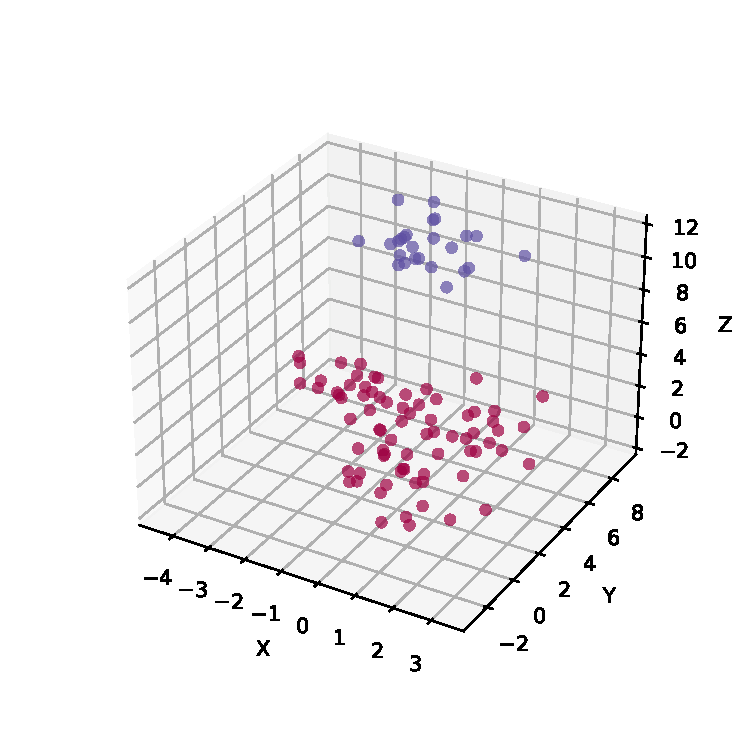
\includegraphics[width=\textwidth]{figures/agglomerative-3d.pdf}
    \caption{}
    \label{fig:agg-3d}
  \end{subfigure}
  \begin{subfigure}{0.45\textwidth}
    \centering
    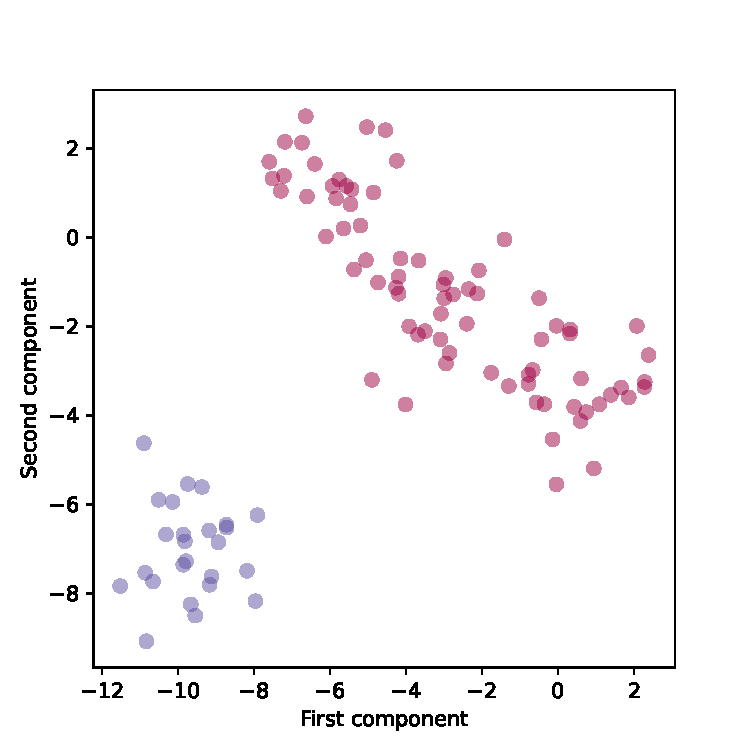
\includegraphics[width=\textwidth]{figures/aglomerative-pca.pdf}
    \caption{}
    \label{fig:agg-pca}
  \end{subfigure}
  \caption[Prueba del algoritmo de agrupamiento aglomerado.]{Prueba del algoritmo de agrupamiento aglomerado. \ref{fig:agg-3d} Visualización sobre los datos sin modificar de los grupos que ha realizado el algoritmo. \ref{fig:agg-pca} Visualización de los grupos realizados sobre los datos procesados por el PCA.}
  \label{fig:agglomerative}
\end{figure}

\newpage
\subsection{Agrupamiento por propagación de afinidad}

El algoritmo de propagación de afinidad \cite{affinity} crea agrupaciones mandando mensajes entre pares de puntos hasta que converge. La principal cualidad de este algoritmo es que, a diferencia con la mayoría de algoritmos de agrupamiento, no necesita saber el número de agrupaciones a realizar de antemano, sino que las genera dinámicamente. Consigue esto ya que, a diferencia de algoritmos como el agrupamiento por k-medias, que inicializa tantos centroides como grupos se quieran obtener, el algoritmo de propagación de afinidad empieza considerando como posibles centroides a todos los puntos de la muestra.

Para ello, el algoritmo se inicializa con una matriz de afinidad $ S $, formada por los valores de afinidad $ s(i, k) $ que indican lo apropiado que sería escoger el dato $ k $ como ejemplar del dato $ i $. Esta matriz puede inicializarse de multitud de formas, pero por defecto se utiliza el negativo de la distancia Euclídea al cuadrado. Con ella, para los puntos $ x_i $, $ x_k $, se tendría
\begin{equation}
  s(i, k) = -||x_i - x_k||^2.
\end{equation}

El algoritmo se ejecuta actualizando dos matrices por medio de \textit{mensajes} hasta que se estabiliza o llega a un número máximo de iteraciones. La \textit{matriz de responsabilidad} $ R $ con valores $ r(i, k) $ cuantifica la evidencia acumulada de como de apropiado es escoger $ x_k $ para ser el ejemplar de $ x_i $. Y la \textit{matriz de disponibilidad} $ A $ con valores $ a(i, k) $ que refleja la evidencia acumulada de como de apropiado sería que un punto $ x_i $ escogiera a un punto $ x_k $ como ejemplar.

Ambas matrices se inicializan a cero y en cada iteración se actualiza primero la matriz de responsabilidad
\begin{equation}
  r(i, k) \leftarrow s(i, k) - \underset{k' \neq k}{\operatorname{max}}\{a(i, k') + s(i, k')\},
\end{equation}
después la matriz de disponibilidad para $ i \neq k $
\begin{equation}
  a(i, k) \leftarrow \operatorname{min}\left\{0, r(k, k) + \sum_{i' \notin \{i, k\}} \operatorname{max}\{0, r(i', k)\}\right\},
\end{equation}
y para el resto de casos
\begin{equation}
  a(k, k) \leftarrow \sum_{i' \neq k} \operatorname{max}\{0, r(i', k)\}.
\end{equation}

Tras alcanzar el criterio de parada se eligen los puntos $ x_k $ para los cuales
\begin{equation}
  a(k, k) + r(k, k) > 0,
\end{equation}
como puntos ejemplares determinando el número de grupos obtenidos y asignando al resto de puntos el grupo de cuyo ejemplar sean más similares.

\begin{mypython}[float={h}, caption={Propagación de afinidad.}, label={code:aff}]
  from sklearn.cluster import AffinityPropagation

  aff = AffinityPropagation()
  aff_assigment = aff.fit_predict(X)
\end{mypython}

En el Código \ref{code:aff} hemos utilizado la clase \texttt{AffinityPropagation} de Scikit-learn para realizar un agrupamiento por propagación de afinidad sobre nuestros datos artificiales. En la Figura \ref{fig:aff} vemos los resultados del agrupamiento, observando como sin haber indicado el número de grupos deseado, el algoritmo consigue diferenciar los cuatro grupos planteados por el generador de datos.

% Affinity
\begin{figure}[h]
  \centering
  \begin{subfigure}{0.45\textwidth}
    \centering
    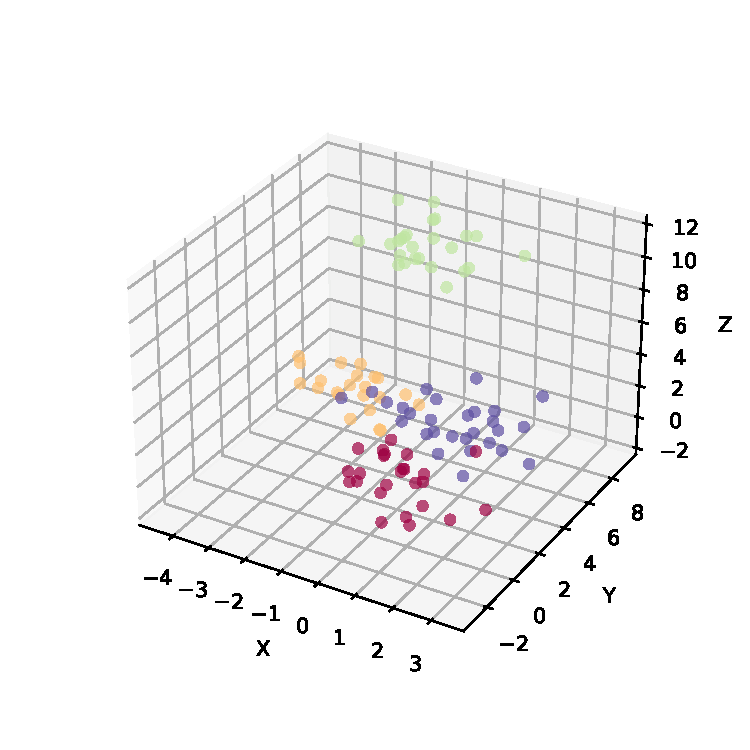
\includegraphics[width=\textwidth]{figures/affinity-3d.pdf}
    \caption{}
    \label{fig:aff-3d}
  \end{subfigure}
  \begin{subfigure}{0.45\textwidth}
    \centering
    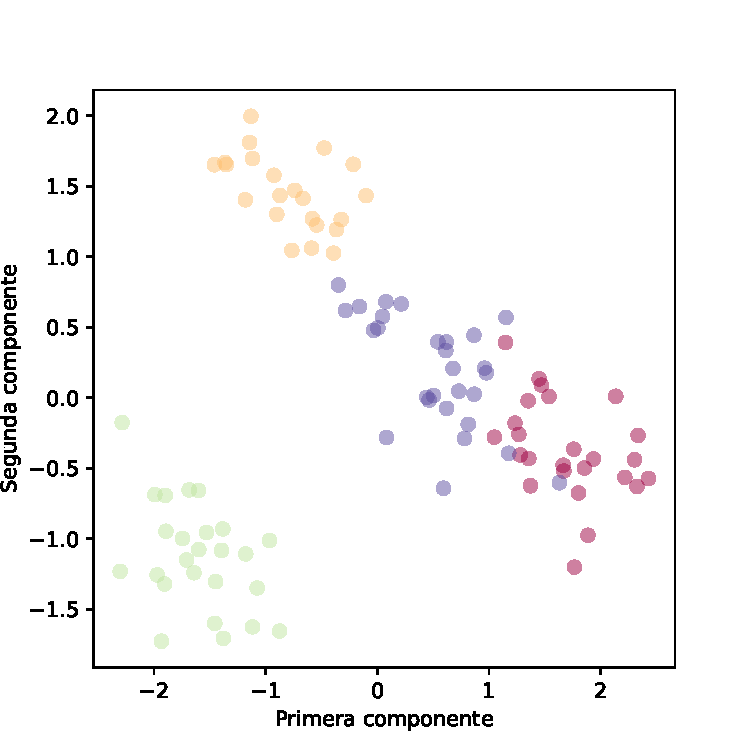
\includegraphics[width=\textwidth]{figures/affinity-pca.pdf}
    \caption{}
    \label{fig:aff-pca}
  \end{subfigure}
  \caption[Prueba del algoritmo de propagación de afinidad.]{Prueba del algoritmo de propagación de afinidad. \ref{fig:aff-3d} Visualización sobre los datos sin modificar de los grupos que ha realizado el algoritmo. \ref{fig:aff-pca} Visualización de los grupos realizados sobre los datos procesados por el PCA.}
  \label{fig:aff}
\end{figure}

\newpage
\section{Métodos supervisados}
\label{sec:supervised}

Al contrario que los métodos de aprendizaje automático no supervisados, donde no sabemos de antemano la salida deseada, los métodos de aprendizaje automático supervisados permiten calibrar los modelos utilizando los datos de salida que queremos mediante el uso de datos de entrenamiento de los cuales conocemos su salida esperada. Para métodos de agrupamiento y separación de clases como los que nos interesan en este trabajo, basta con contar con un conjunto de datos previamente etiquetado con su clase real como datos de entrenamiento, permitiendo a los modelos aprender sobre la clasificación dada y posteriormente replicarla para datos nuevos.

\cite{pytorch}

\subsection{Red neuronal secuencial}

% Net
\begin{figure}[h]
  \centering
  \begin{subfigure}{0.45\textwidth}
    \centering
    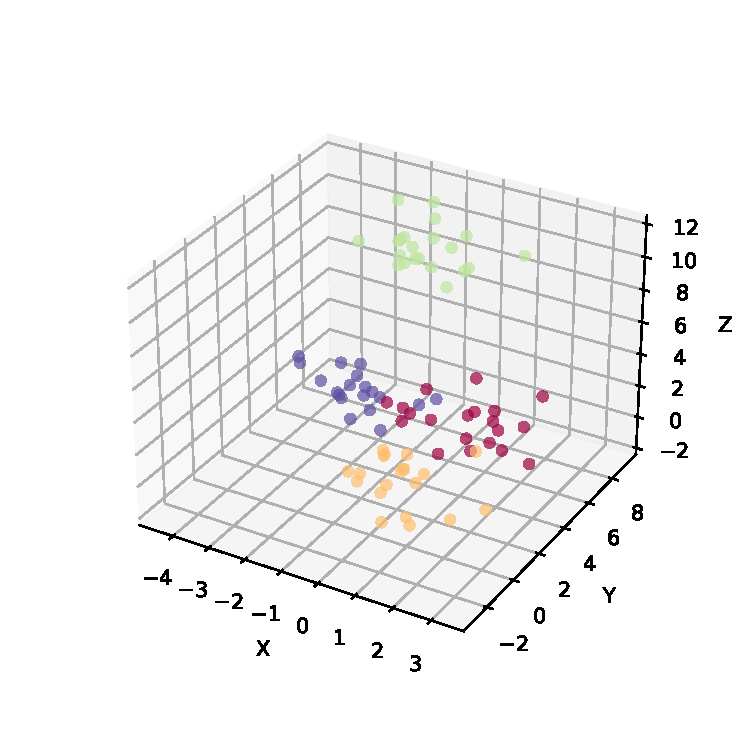
\includegraphics[width=\textwidth]{figures/train-asig-artificial.pdf}
    \caption{}
    \label{fig:}
  \end{subfigure}
  \begin{subfigure}{0.45\textwidth}
    \centering
    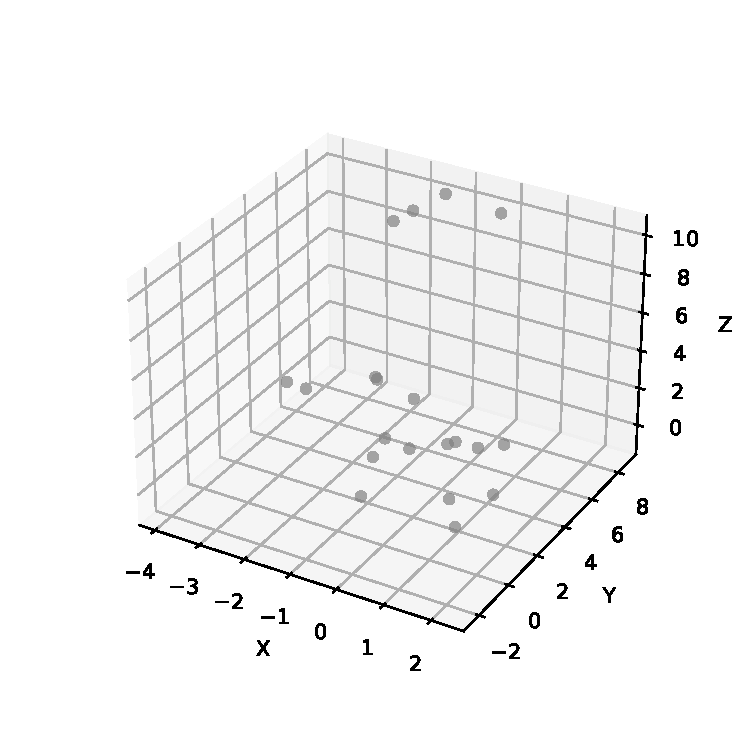
\includegraphics[width=\textwidth]{figures/test-artificial.pdf}
    \caption{}
    \label{fig:}
  \end{subfigure}
  \begin{subfigure}{0.45\textwidth}
    \centering
    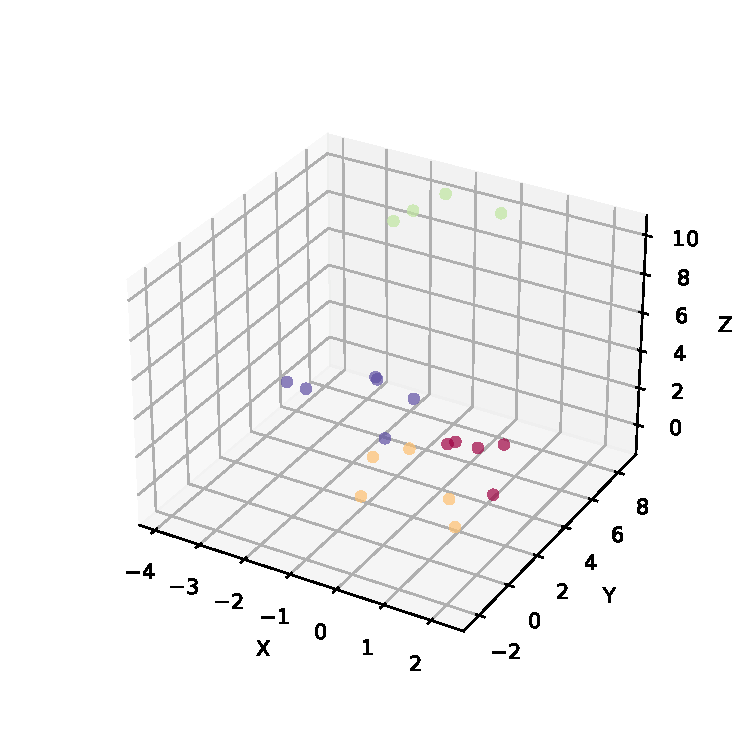
\includegraphics[width=\textwidth]{figures/test-asig-artificial.pdf}
    \caption{}
    \label{fig:}
  \end{subfigure}
  \caption[Prueba de red neuronal secuencial.]{}
  \label{fig:}
\end{figure}

\subsection{Red neuronal convolucional}